En este capítulo se trata el entendimiento del problema o dominio. Tal y como se comenta en el Capítulo \ref{cap.metodologia}, es la fase inicial de la metología CRISP-DM. A continuación, se alinean los objetivos técnicos con las necesidades del negocio y con el problema a resolver. Se definen requisitos, se identifican métricas de éxito y se trata de dar comprensión sobre el contexto organizacional. La totalidad de la fase de entendimiento del problema de la metodología usada, se distribuye entre este capítulo, el Capítulo \ref{cap.introduccion}, donde se fijan los objetivos del proyecto y el Capítulo \ref{cap.req-planificacion}, donde se establece la planificación y los riesgos.


\section{¿Qué es un ataque a un sistema informático?}
Un ataque a un sistema informático constituye una acción deliberada y no autorizada que explota vulnerabilidades con el objetivo de comprometer la confidencialidad, integridad o disponibilidad de los datos y recursos del sistema. Esta actividad maliciosa puede manifestarse a través de diversas técnicas, incluyendo la inyección de código malicioso, la denegación de servicio, el acceso no autorizado y la ingeniería social. Su ejecución busca obtener beneficios ilícitos, interrumpir operaciones o dañar la infraestructura tecnológica \cite{ethical_hacking}.

La consecuencia de un ataque puede variar desde la pérdida o alteración de información sensible hasta la paralización completa de los servicios ofrecidos por el sistema. La identificación, análisis y mitigación de estas amenazas representan un aspecto fundamental en la seguridad informática, requiriendo la implementación de medidas preventivas y reactivas para proteger los activos digitales de una organización o individuo \cite{conataques}.

\section{Tipos de ataque a sistemas informáticos}
Los ataques a sistemas informáticos se pueden clasificar de distintas maneras según su naturaleza. A continuación, se detallan los más comunes y peligrosos:

\begin{itemize}

\item{\textbf{Ataques de Denegación de Servicio (DoS)}}.
Un ataque de Denegación de Servicio tiene como objetivo hacer que un sistema o red no esté disponible para sus usuarios legítimos, interrumpiendo su funcionamiento normal. Estos ataques se llevan a cabo sobrecargando los recursos de un servidor o red con una cantidad excesiva de solicitudes. Un ejemplo de este tipo de ataque es el Ataque de Denegación de Servicio Distribuido (DDoS), en el cual múltiples dispositivos comprometidos atacan al mismo tiempo un servidor, sobrecargándolo hasta que se vuelve inoperativo \cite{tanenbaum2009}.


\item{\textbf{Ataques de Inyección}}.
Los ataques de inyección ocurren cuando un atacante introduce código malicioso en un sistema que no valida correctamente las entradas de los usuarios. Un ejemplo común es la inyección SQL, donde un atacante puede insertar comandos SQL en una aplicación web para acceder, modificar o eliminar datos en una base de datos. Este tipo de ataque explota la falta de medidas de validación y filtrado en las entradas del sistema \cite{scott2015}.

\item{\textbf{Ataques de \textit{Phishing}}}.
El \textit{phishing} es un tipo de ataque en el que un atacante engaña a una persona para que proporcione información confidencial, como contraseñas o detalles bancarios. Generalmente, esto se realiza mediante correos electrónicos o sitios web fraudulentos que simulan ser una entidad de confianza, como bancos o servicios en línea. La principal característica del \textit{phishing} es la manipulación psicológica de la víctima \cite{cissp2018}.

\item{\textbf{Ataques de \textit{Malware}}}.
El \textit{malware} es un software malicioso diseñado para dañar o robar información de un sistema informático. Entre los tipos más comunes de \textit{malware} se encuentran los virus, gusanos, troyanos y \textit{ransomware}. El \textit{ransomware}, por ejemplo, cifra los archivos de un sistema y exige un pago para liberar el acceso a los mismos. Los ataques de \textit{malware} pueden ser ejecutados a través de archivos adjuntos de correo electrónico, descargas de software malicioso o vulnerabilidades de seguridad.

Los ataques de \textit{Malware} que se tratan en este trabajo son: \textit{Backdoor} y \textit{Worms}.

\item{\textbf{Ataques \textit{Man-in-the-Middle} (MitM)}}.
En un ataque \textit{Man-in-the-Middle} (de intermediario o de hombre en el medio), el atacante intercepta y, a veces, modifica la comunicación entre dos partes sin que ellas lo sepan. Estos ataques son comunes en redes no seguras, como las redes Wi-Fi públicas. El atacante puede obtener información confidencial, como contraseñas y datos de tarjetas de crédito, si no se utilizan medidas de seguridad adecuadas, como cifrado de las comunicaciones \cite{tanenbaum2009}.

\item{\textbf{\textit{Exploits} de Vulnerabilidades}}.
Un \textit{exploit} es un ataque que se aprovecha de una vulnerabilidad en el software o hardware de un sistema. Estos ataques se basan en el aprovechamiento de fallos conocidos en programas o dispositivos sin que el fabricante o el usuario los haya corregido. Los \textit{exploits} pueden permitir a los atacantes ejecutar código malicioso en un sistema, obtener acceso a información confidencial o incluso tomar control total de la máquina afectada \cite{cissp2018}.

Aquellos ataques que pertenecen al tipo \textit{Exploits} de vulnerabilidades que el modelo de clasificación multiclase deberá distinguir son: \textit{Fuzzers}, \textit{Exploits} y \textit{Shellcode}.

\end{itemize}

\section{¿Qué es TCP?}

El Protocolo de Control de Transmisión (\textit{Transmission Control Protocol}, TCP) constituye uno de los protocolos fundamentales de la capa de transporte del modelo TCP/IP, sobre el cual se sustenta gran parte de la comunicación en redes IP, incluyendo Internet. Su diseño se orienta a proporcionar un servicio de transferencia de datos fiable, ordenado y con detección de errores entre aplicaciones que se ejecutan en sistemas finales diferentes. Para lograr esta fiabilidad, TCP establece una conexión virtual punto a punto entre las aplicaciones comunicantes mediante un proceso de \textit{three way handshake} (triple apretón de manos) que se muestra en la Figura \ref{fig:EsquemaTCP}, lo que permite la negociación de parámetros de la conexión y la sincronización de los números de secuencia iniciales.

\begin{figure}[htbp]
    \centering
    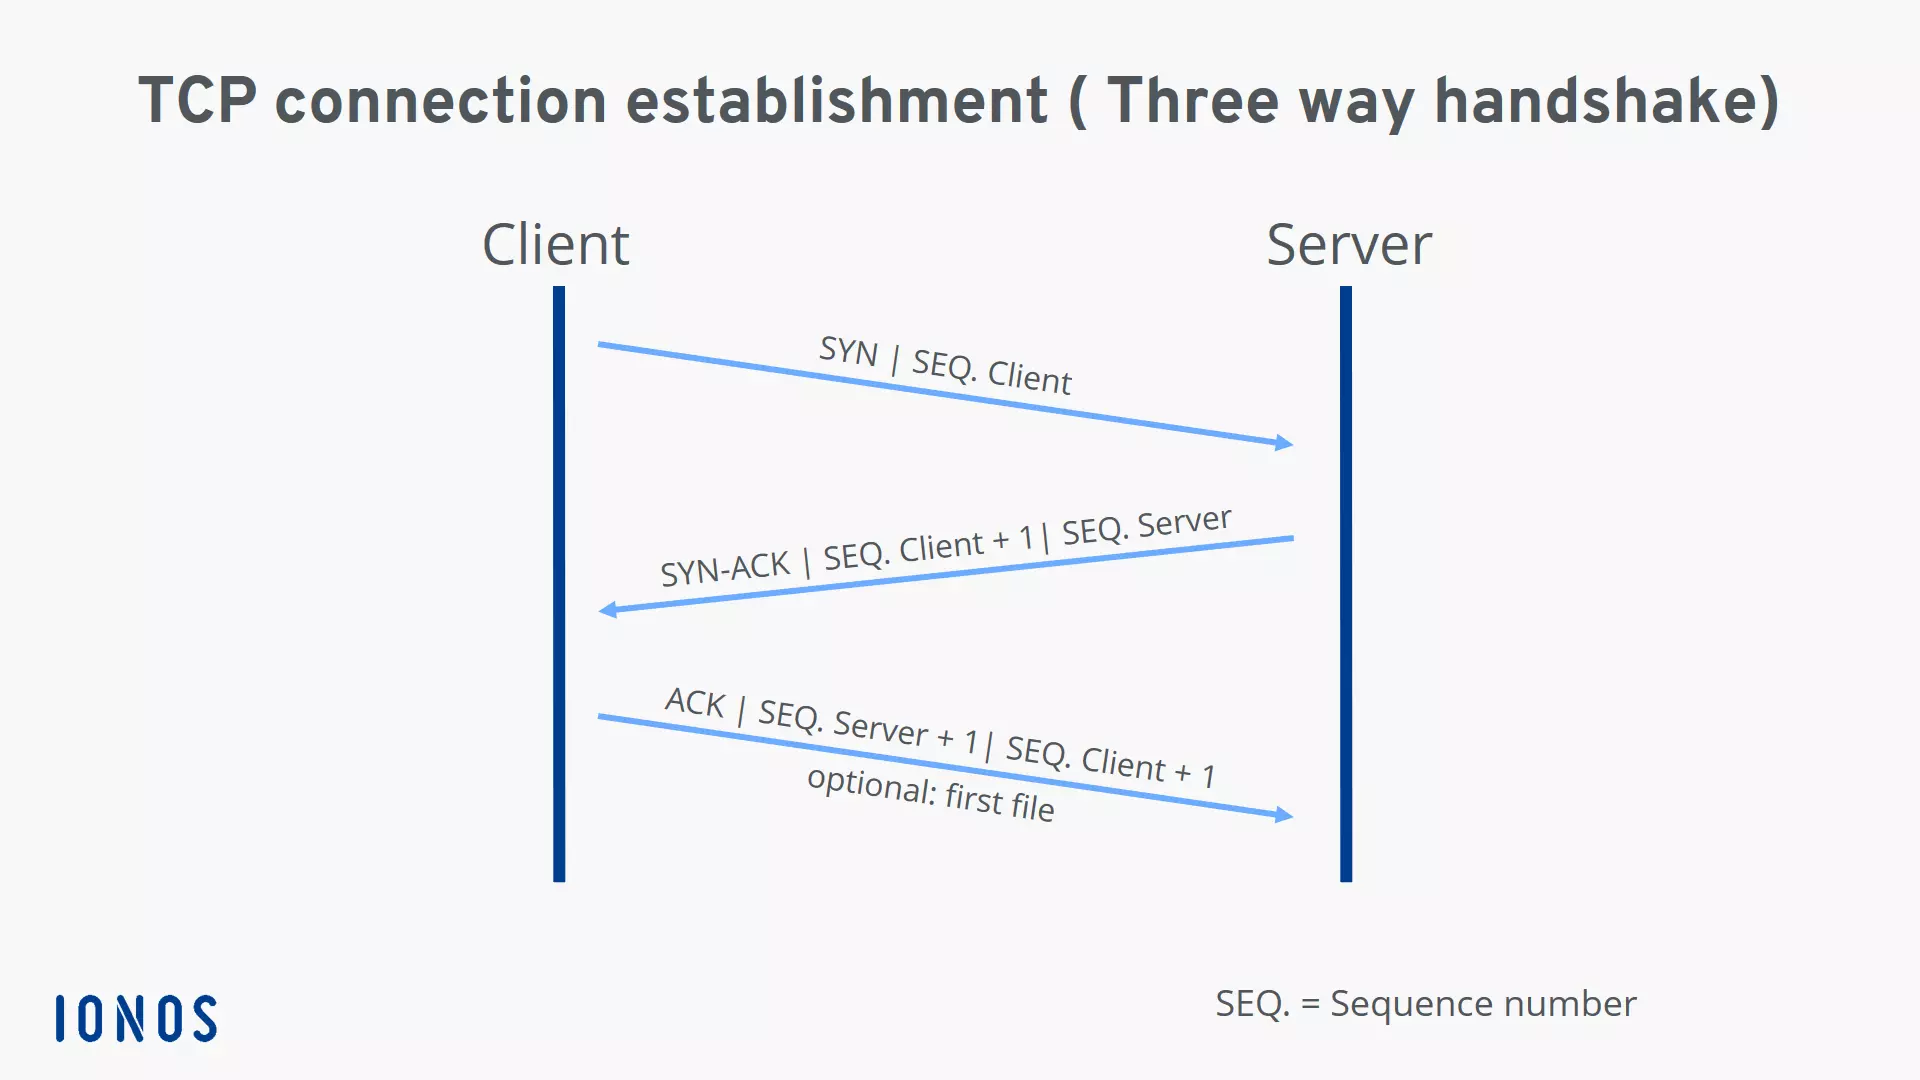
\includegraphics[width=0.8\textwidth]{./img/ent-problema/EsquemaTCP.png}
    \caption{Esquema del \textit{three way handshake} de TCP \cite{tcpprotocolionos}.}
    \label{fig:EsquemaTCP}
\end{figure}

El protocolo garantiza la entrega ordenada de la información al receptor mediante la asignación de números de secuencia a cada byte transmitido, permitiendo así la reordenación en caso de que la información no llegue al receptor en el orden correcto. La fiabilidad se logra a través de un mecanismo de acuse de recibo (\textit{acknowledgment}, ACK) positivo con retransmisión, donde el receptor confirma la recepción correcta de los paquetes de información, y el emisor retransmite aquellos partes de la información para los que no recibe confirmación dentro de un tiempo límite (\textit{timeout}).

\subsection{¿Qué es un segmento TCP?}
Una vez establecida la conexión, TCP divide los datos de la aplicación en unidades más pequeñas denominadas segmentos cuya estructura se detalla en la Figura \ref{fig:SegmentoTCP}. Un segmento o paquete TCP constituye la unidad de datos fundamental que se intercambia a través de una red utilizando el mencionado protocolo TCP. Este segmento encapsula una porción de los datos de la capa de aplicación, precedida por una cabecera TCP. 

La cabecera TCP contiene información de control esencial para la funcionalidad del protocolo, incluyendo los números de puerto de origen y destino que identifican las aplicaciones comunicantes, los números de secuencia y de acuse de recibo ACK que garantizan la entrega ordenada y fiable, las banderas de control que indican el propósito del segmento (establecimiento de conexión, finalización, ACK, entre otros muchos), y otros campos como la ventana de recepción para el control de flujo y la suma de verificación para la detección de errores.


\begin{figure}[H]
    \centering
    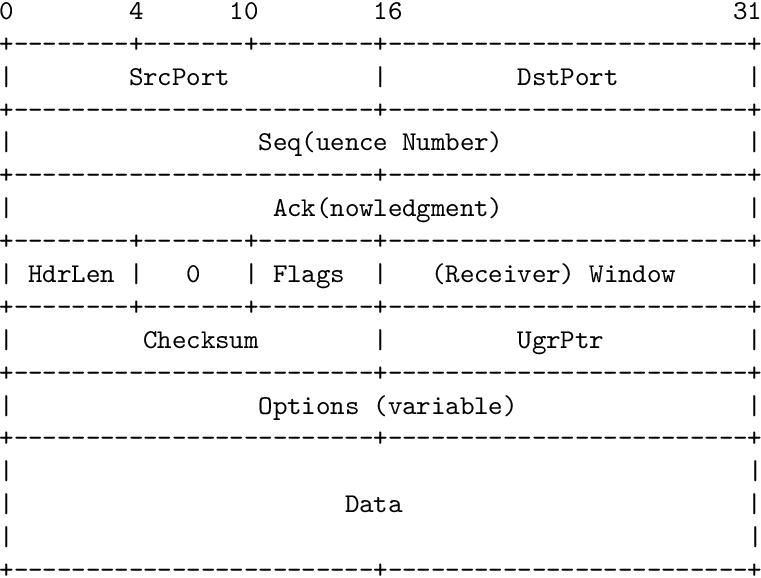
\includegraphics[width=0.8\textwidth]{./img/ent-problema/SegmentoTCP.png}
    \caption{Esquema segmento TCP \cite{tcpsegment}.}
    \label{fig:SegmentoTCP}
\end{figure}

En el proceso de transmisión, el segmento TCP se encapsula a su vez dentro de un paquete IP (Protocolo de Internet) para su enrutamiento a través de la red. El paquete IP añade su propia cabecera con las direcciones IP de origen y destino, entre otra información necesaria para el transporte a nivel de red. Toda esta estructura se puede observar con detalle en la Figura \ref{fig:PaqueteIP}.

\begin{figure}[H]
    \centering
    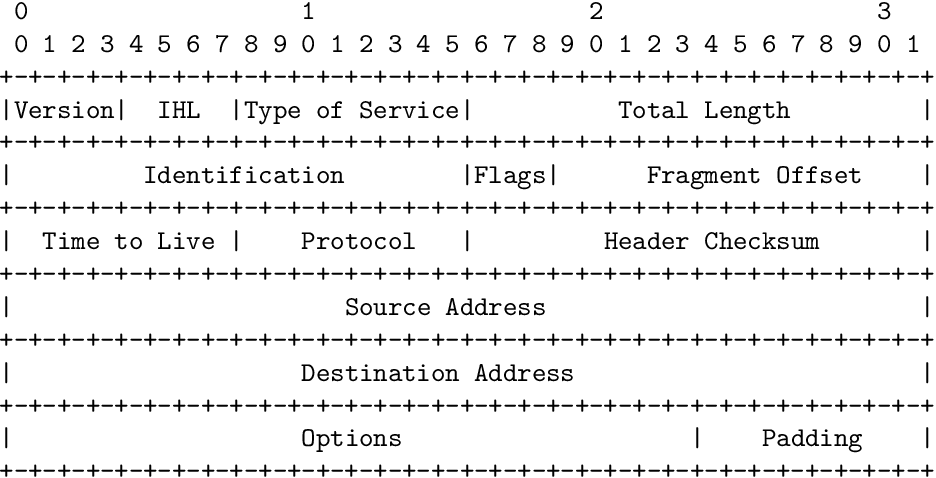
\includegraphics[width=0.8\textwidth]{./img/ent-problema/PaqueteIP.png}
    \caption{Formato de la cabecera en IPv4 \cite{paqueteip}.}
    \label{fig:PaqueteIP}
\end{figure}

\section{Importancia de protegerse frente a un ataque}

La importancia de protegerse frente a ataques informáticos radica en la salvaguarda de activos digitales críticos, la garantía de la continuidad operativa y la preservación de la confianza y la reputación. En un entorno digital cada vez más interconectado, los ataques informáticos representan una amenaza significativa para individuos, organizaciones y la sociedad en su conjunto, pudiendo acarrear consecuencias devastadoras \cite{Santos2020}.

Para las organizaciones, las implicaciones de un ataque informático pueden ser aún más costosas. Estas implicaciones incluyen pérdidas financieras directas debido al robo de fondos, la interrupción de las operaciones comerciales, los costes de recuperación y las posibles sanciones regulatorias. Además, se puede producir un daño significativo a la reputación y la pérdida de la confianza de los clientes, lo que a largo plazo afecta la viabilidad del negocio. Los ataques también pueden resultar en el robo de propiedad intelectual, secretos comerciales e información estratégica, otorgando ventajas competitivas a adversarios \cite{Ponemon2019}. 

Por otra parte, la interrupción de servicios críticos, como energía, comunicaciones o sanidad, puede tener consecuencias graves para la sociedad en su conjunto.

La protección frente a ataques informáticos no es solo una cuestión de seguridad tecnológica, sino una necesidad imperante en la actualidad para proteger activos valiosos, asegurar la continuidad de las actividades, mantener la confianza de los usuarios y garantizar la estabilidad y el bienestar en el mundo digital actual. La implementación de prácticas de seguridad robustas y la concienciación sobre las amenazas cibernéticas son fundamentales en a la hora de defenderse de estos ataques \cite{Bada2017}.


\section{Importancia de detectar los ataques rápidamente}

La detección temprana de ataques informáticos constituye un pilar fundamental en la ciberseguridad moderna debido a su capacidad para mitigar consecuencias críticas. Cuando un sistema logra identificar intrusiones o actividades maliciosas en sus fases iniciales, se reducen significativamente los daños operativos y económicos. Esta rapidez de respuesta permite contener amenazas antes de que comprometan infraestructuras completas, preservando tanto la integridad de los datos como la continuidad del negocio \cite{anderson2020}.

Desde una perspectiva técnica, la identificación inmediata limita la superficie de ataque, impidiendo que los actores maliciosos escalen privilegios o se propaguen lateralmente por la red. En el ámbito regulatorio, cumple con los estrictos plazos que exigen normativas como el Reglamento General de Protección de Datos (RGPD) \cite{RGPD2016}, que obliga todos los paises miembros de la Unión Europea a notificar violaciones de seguridad en un máximo de 72 horas. Esta normativa fue promovida por la Unión Europea con el objetivo de fortalecer y unificar la protección de los datos personales en todo el territorio de la UE. El RGPD entró en vigor el 25 de mayo de 2018, después de un período de transición de dos años para que las organizaciones pudieran adaptarse a las nuevas normativas. Además, desde el punto de vista económico, reduce los costes asociados a las reparaciones, que suelen multiplicarse exponencialmente cuando los ataques permanecen indetectados durante largos períodos.


La capacidad de detectar rápidamente anomalías en el tráfico de red, accesos no autorizados o patrones de comportamiento sospechosos no solo protege los activos digitales, sino que también salvaguarda la reputación institucional. Organizaciones con sistemas de detección temprana robustos demuestran proactividad ante clientes y socios comerciales, generando confianza en su capacidad para manejar información sensible. Esta anticipación resulta especialmente crítica en entornos donde la disponibilidad del servicio es primordial, como en las infraestructuras críticas anteriormente mencionadas \cite{Sommestad2019}.

\section{Soluciones comerciales o actuales a estos problemas}

En esta sección se comentan algunas de las soluciones y software que se utilizan en la actualiadad para detectar y neutralizar posibles ataques informáticos. Estas herramientas protegen los sistemas informáticos analizando y controlando el tráfico de la red.

Los \textit{firewalls} de próxima generación (NGFW) como Palo Alto Networks, Check Point o Cisco Firepower, inspeccionan el tráfico de red a un nivel profundo (Deep Packet Inspection - DPI), analizando el contenido de los paquetes más allá de los puertos y protocolos tradicionales. Este enfoque se sustenta en diversas tecnologías avanzadas, incluyendo técnicas de inteligencia artificial (IA) y aprendizaje automático (ML), que permiten una detección más precisa y dinámica de amenazas. Palo Alto Networks, por ejemplo, emplea IA a través de su sistema \textit{WildFire}, que utiliza análisis de comportamiento y \textit{sandboxing} para identificar \textit{malware} y amenazas avanzadas. Por su parte, Check Point implementa el uso de \textit{ThreatCloud}, una plataforma que aplica algoritmos de IA para la detección y prevención de amenazas, y que se beneficia de la inteligencia colectiva de miles de dispositivos conectados. Cisco Firepower se apoya en tecnologías de \textit{next-generation IPS} y \textit{URL filtering}, además de usar análisis de tráfico basado en IA para identificar patrones anómalos de tráfico y potenciales riesgos de seguridad. Estas herramientas permiten identificar y bloquear amenazas sofisticadas, \textit{malware}, y tráfico de aplicaciones maliciosas, además de ofrecer funcionalidades como prevención de intrusiones (IPS) y control de aplicaciones \cite{cosmikal_firewall}.


Los sistemas de detección y prevención de intrusiones o IDS e IPS, como: \textit{Snort}, \textit{Suricata} o \textit{Trend Micro TippingPoint}, monitorean el tráfico de red en tiempo real en busca de patrones sospechosos o firmas de ataques conocidos. Los IDS alertan sobre posibles intrusiones, mientras que los IPS tienen la capacidad de bloquear o mitigar activamente el tráfico malicioso detectado, interrumpiendo los ataques en curso. Estas herramientas emplean diversas tecnologías para el análisis del tráfico y la detección de amenazas. \textit{Snort}, por ejemplo, se basa en un sistema de detección de firmas y anomalías, utilizando algoritmos de análisis de tráfico que, aunque tradicionalmente no utilizan IA, han sido extendidos con módulos que incorporan técnicas de aprendizaje automático para mejorar su capacidad de identificar ataques desconocidos. \textit{Suricata}, por su parte, también emplea un sistema de detección basado en firmas y análisis de flujo, pero se distingue por su capacidad para procesar grandes volúmenes de tráfico en paralelo, y su integración con herramientas de análisis de inteligencia de amenazas que utilizan IA para mejorar la precisión en la identificación de ataques avanzados. \textit{Trend Micro TippingPoint} utiliza un enfoque de prevención de intrusiones de próxima generación que integra tecnologías de inspección profunda de paquetes (\textit{DPI}) y análisis de tráfico en tiempo real, además de implementar IA y aprendizaje automático para detectar patrones de comportamiento anómalo y bloquear ataques sofisticados \cite{geekflare_ids_ips}.

La microsegmentación de red con herramientas como VMware NSX, Cisco ACI o Illumio, divide la red en segmentos más pequeños y aislados, aplicando políticas de seguridad granular a cada segmento. Esto limita el movimiento lateral de los atacantes dentro de la red una vez que han comprometido un punto inicial. Al controlar el tráfico entre estos segmentos, se reduce la superficie de ataque y se contiene la propagación de las amenazas \cite{paloaltonetworks_microsegmentation}.

\section{Requisitos}  \label{sec.requisitos} 
En la fase de entendimiento del problema de la metodología CRISP-DM es fundamental establecer claramente los requisitos que se deben cumplir durante el desarrollo del proyecto. Para definir los requisitos se ha utilizado el estándar ISO/IEC/IEEE 29148:2018 \cite{ISO29148} que trata sobre ingeniería de requisitos en sistemas y software. Este estándar especifica los procesos necesarios para desarrollar requisitos a lo largo del ciclo de vida de un proyecto o sistema.

Como se ha comentado en la Sección \ref{sec.objetivos-pro} \nameref{sec.objetivos-pro}, el principal objetivo del proyecto es desarrollar un modelo neuronal que detecte la presencia de ataques en una red informática y los clasifique según su tipo. Para cumplir con dicho objetivo, se considera imprescindible cumplir con los requisitos que se listan a continuación.

\subsection{Requisitos Funcionales}   \label{sec.req-funcionales}

\begin{itemize}  
    \item \textbf{RF-1}: El sistema deberá detectar cuales de las conexiones podrían ser potenciales intrusiones en la red.
    \item \textbf{RF-2}: El sistema deberá clasificará las conexiones en 10 categorías predefinidas en \ref{tab:attacks-tab} \nameref{tab:attacks-tab}.  
	\item \textbf{RF-3}: El sistem deberá ser capaz de procesar formatos estándar de logs como son Syslog, NetFlow y PCAP.
	\item \textbf{RF-4}: El sistema deberá diferenciar entre ataques conocidos (basados en firmas) y desconocidos (basados en anomalías).
	%\item \textbf{RF-5}: El sistema deberá ofrecer API REST para conexión con SIEMs (Splunk, IBM QRadar).
	%\item \textbf{RF-6}: Generar alertas automatizadas con nivel de criticidad (bajo/medio/alto).
	%\item \textbf{RF-7}: Proveer recomendaciones de mitigación básicas (ej. bloquear IPs maliciosas).
	
\end{itemize}  

\subsection{Requisitos No Funcionales}   \label{sec.req-no-funcionales}
\begin{itemize}  
    \item \textbf{RNF-1}: Latencia $<$50 ms en redes de 10Gbps (requisito crítico para SOC~\cite{nist2021ai}).  
    \item \textbf{RNF-2}: Interfaz accesible para usuarios no técnicos (evaluado con test SUS~\cite{brooke1996sus}).
    \item \textbf{RNF-3}: Se debe utilizar el \textit{dataset} \texttt{NF-UNSW-NB15-v3} para entrenar los modelos.  
\end{itemize}  
